% !TEX root = ../../../main.tex

\begin{figure}[!htb]
    \centering
    \begin{subfigure}{0.31\textwidth}
        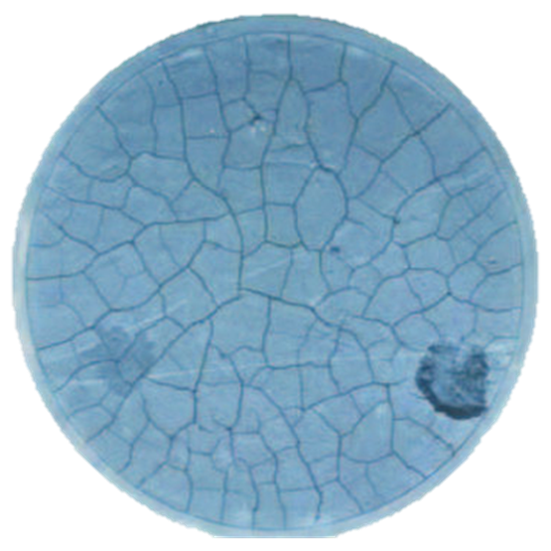
\includegraphics[width=\textwidth,scale=0.5]{past/figures/4mm_exp.png}
    \end{subfigure}
    \begin{subfigure}{0.31\textwidth}
        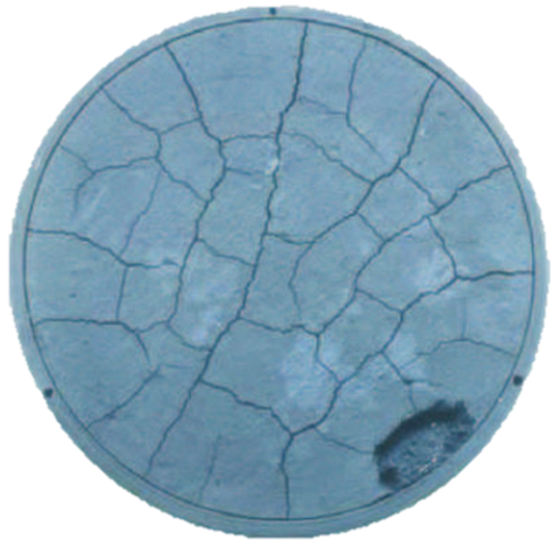
\includegraphics[width=\textwidth,scale=0.5]{past/figures/8mm_exp.png}
    \end{subfigure}
    \begin{subfigure}{0.31\textwidth}
        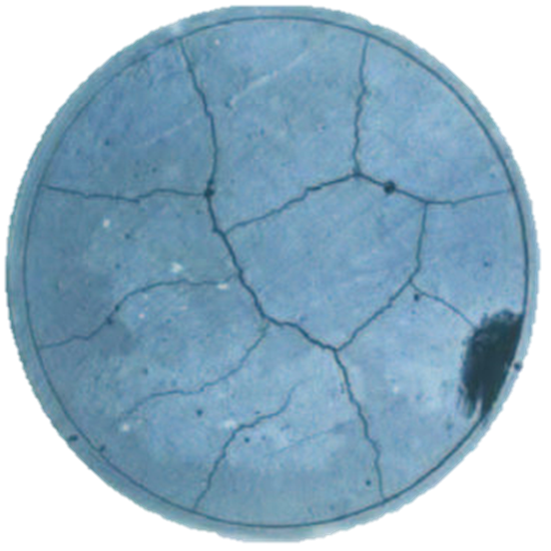
\includegraphics[width=\textwidth,scale=0.5]{past/figures/16mm_exp.png}
    \end{subfigure}

    \begin{subfigure}{0.31\textwidth}
        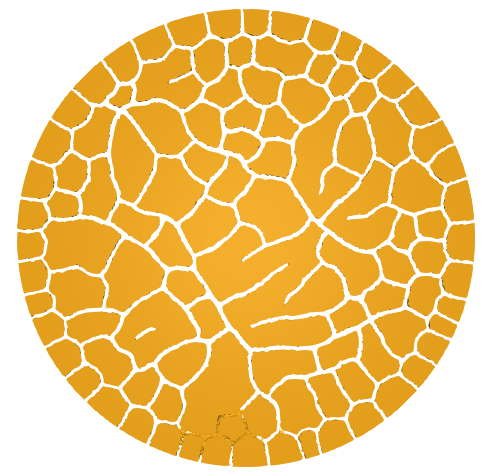
\includegraphics[width=\textwidth,scale=0.5]{past/figures/4mm_top.png}
    \end{subfigure}
    \begin{subfigure}{0.31\textwidth}
        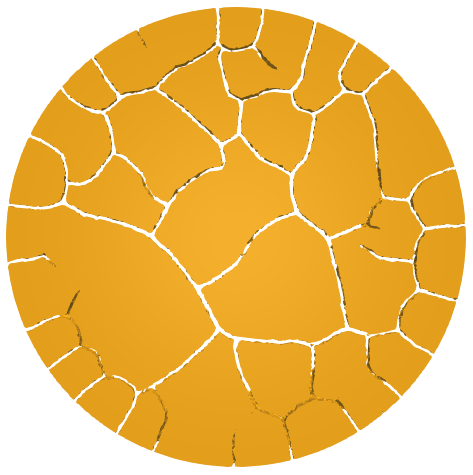
\includegraphics[width=\textwidth,scale=0.5]{past/figures/8mm_top.png}
    \end{subfigure}
    \begin{subfigure}{0.31\textwidth}
        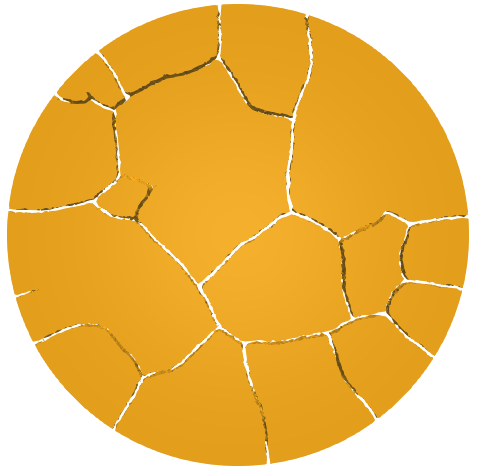
\includegraphics[width=\textwidth,scale=0.5]{past/figures/16mm_top.png}
    \end{subfigure}

    \begin{subfigure}{0.31\textwidth}
        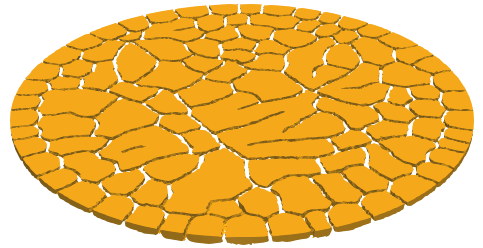
\includegraphics[width=\textwidth,scale=0.5]{past/figures/4mm_3D.png}
    \end{subfigure}
    \begin{subfigure}{0.31\textwidth}
        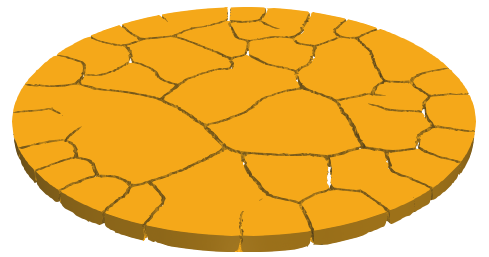
\includegraphics[width=\textwidth,scale=0.5]{past/figures/8mm_3D.png}
    \end{subfigure}
    \begin{subfigure}{0.31\textwidth}
        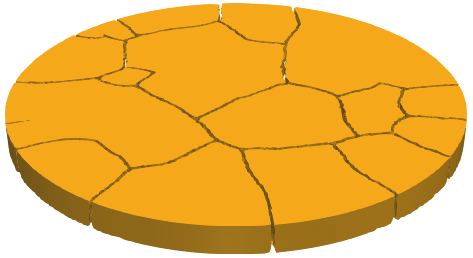
\includegraphics[width=\textwidth,scale=0.5]{past/figures/16mm_3D.png}
    \end{subfigure}
\end{figure}
